% LaTeX template for URSI Radio Science Letters (RSL)
%
% Use pdflatex or latex + dvips + ps2pdf to produce a PDF.
%
% 15 June 2021, Henrik Wallen <henrik.wallen@aalto.fi>

%
% Submissions to RSL must use the default class option [manuscript].
% At other stages the [preprint] option can be handy.
%
\documentclass[preprint]{rsl}
%\documentclass{rsl}

%
% DO NOT add any packages or define custom macros.
%

% Title and author(s)
%
% Use explicit line-breaks \\ if needed and note that the affiliations are
% at the end of the manuscript.
%
\title{On-Body Path Loss Modeling in the 110 to 170~GHz Range}
\author{Brecht De Beelde,
Reza~Aminzadeh,
Arno~Thielens,
Wout~Joseph
}

\begin{document}

\maketitle

%
% Manuscript contents begins.
%

\begin{abstract}
This letter presents empirical on-body path loss (PL) models for radio-frequency electromagnetic fields (RF-EMFs) at frequencies in the D-band, ranging from 110 to 170~GHz. 
PL is measured for distances ranging from 1 to 19~cm using a vector network analyzer (VNA)-based channel sounder with frequency extenders and using vertically and horizontally polarized horn antennas placed at heights of 1~mm to 6~mm above a skin phantom.
The measured PL is fitted to an alpha-beta-gamma model, and wideband PL is fitted to a floating-intercept model.
Both models have a high reference PL and low PL exponent below 1. 
Even though the frequency dependence is small, PL increases with frequency. 
When the antennas are closer to the skin phantom, more electromagnetic power is absorbed by the phantom which results in a higher PL.
\end{abstract}

\section{Introduction\label{sect:intro}}

In the last decade, the domain of personal area networks (PAN) has evolved into wireless body area networks (WBANs), where sensor and actuator nodes in and on the body  wirelessly transmit data to eachother \cite{Patel2010,Reusens2009} or off the body \cite{Marinova2015}. 
Numerous channel models for WBANs at frequencies below 10~GHz are available \cite{VanRoy2010,Qaraqe2014} and WBANs operational at millimeter-wave frequencies are being deployed, e.g., using the 60~GHz industrial, scientific, and medical (ISM) frequency band \cite{Chahat2013,Petrillo2014,Aminzadeh2021_tap}, and the W-band around 94 GHz \cite{Brizzi2013,Ali2022}.

On-body PL is generally studied using three approaches: theoretically \cite{Chahat2013,Petrillo2014}, numerically \cite{Reusens2009}, and using measurements \cite{Chahat2013,Reusens2009,Aminzadeh2021_tap}. 
On-body measurements have the disadvantages that they introduce subject-to-subject variation \cite{Proesmans2022} and that it is difficult for a subject to remain immobile. 
Therefore, human-body mimicking objects, so-called phantoms, are used to stabilize and standardize these measurements \cite{Chahat2013}. 
Apart from research on radio propagation near the body, the design of antennas for WBAN applications is an active research topic \cite{Zhang2021,Mahmood2020,Hong2016,Tak2016,Verbiest2006}.
It is envisioned that future communication systems, including sixth generation (6G) wireless networks, will be important for the realization of WBANs \cite{Cornet2022}, for example in applications such as wireless prosthetics where large data rates need to be achieve over relatively short separation distances \cite{Proesmans2022}.
These future communication systems may use frequencies above 100~GHz, such as the D-band with frequencies ranging from 110 to 170~GHz.
D-band channel models are available for indoor \cite{DeBeelde2021_access, Pometcu2020} and outdoor \cite{DeBeelde2022_tap,DeBeelde2022_wcl} environments. 
In this work, we present an on-body path loss (PL) model for D-band frequencies. 
For the first time, on-phantom PL measurements are performed above 100~GHz with the goal to characterize the radio channel for short-range high-data rate wireless communication in WBANs.
Compared to the existing D-band models, not only is the presence of the skin near the Line-of-Sight (LOS) path important, but the antenna separation limited as well. 


% The outline of this letter is as follows.
% Section~\ref{sect:method} provides the measurement setup and scenarios. 
% Section~\ref{sect:results} provides the measurement results and path loss models, and Section~\ref{sect:conclusion} concludes this letter.

\section{Methodology \label{sect:method}}

A vector network analyzer (VNA) with frequency extenders is used to perform D-band channel measurements for antenna separations up to 19~cm, with a skin phantom positioned between the antennas.
In the remainder of this letter, we will refer to on-body PL measuremements when the skin phantom is present near the antennas. 
This measurement setup is presented in Fig.~\ref{fig:sounder_setup}.
\begin{figure}[tb]
\begin{center}
	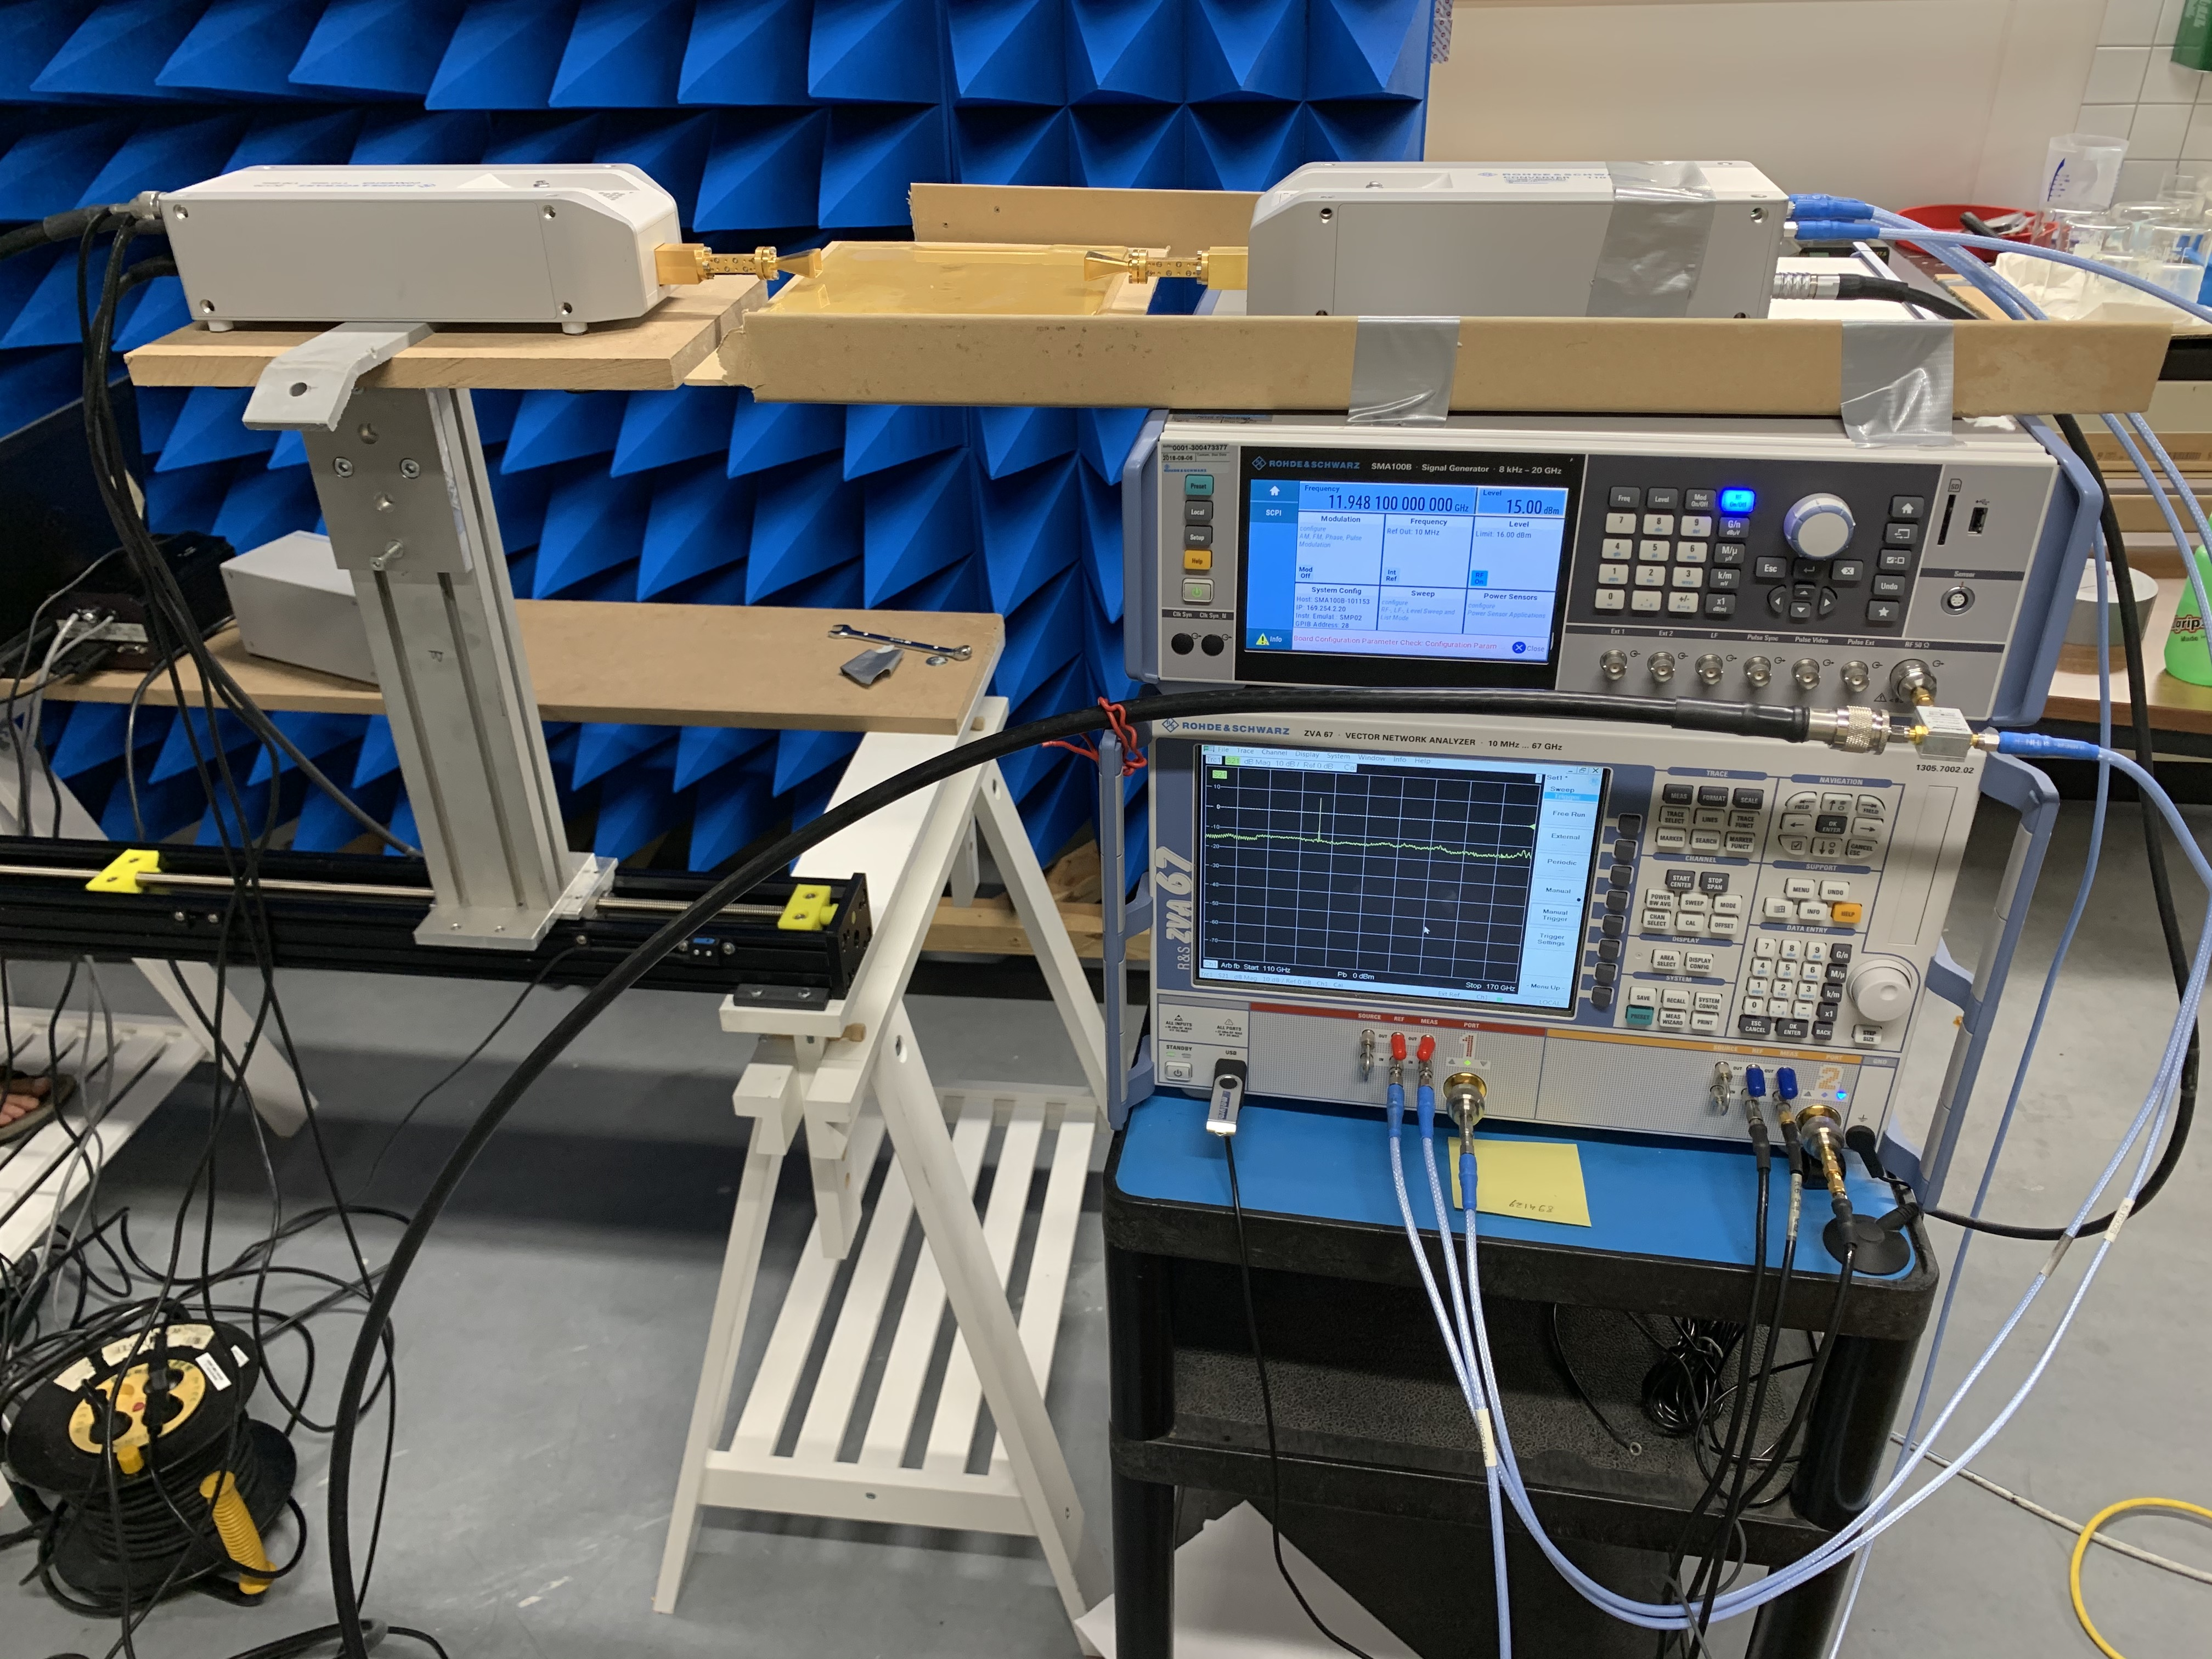
\includegraphics[width=0.45\textwidth]{figures/measurement_setup}
\caption{The measurement setup with a vector network analyzer (VNA)-based channel sounder.}
\label{fig:sounder_setup}
\end{center}
\end{figure}

\subsection{Channel sounder}

The VNA generates a radio frequency (RF) source input that is multiplied via frequency multiplication using an external frequency up-converter, which results in an RF output in the frequency range 110 to 170~GHz. 
A harmonic mixer with a multiplication factor of 10 and a local oscillator (LO) input in the frequency range 11 to 17~GHz are used for down-conversion to generate a reference signal for the VNA. 
A standard gain pyramidal horn antenna with a gain increasing from 22.2~dBi for 110~GHz  to 23.3~dBi for 170~GHz is connected to the frequency converter's WR-6 waveguide and transmits the D-band signal.
At the receiver side, an identical antenna captures the received signal, which is down-converted using the harmonic mixer of the frequency down-converter that uses the same LO input. 
The down-converted signal is sent to the measurement port of the VNA. 
The VNA measures the phase and amplitude difference between the reference signal at port 1 and the measured signal at port 2.
The antennas have an H-plane half power beam width (HPBW) ranging from 13.2$^{\circ}$ at 110~GHz to 12$^{\circ}$ at 170~GHz and an E-plane HPBW ranging from 12$^{\circ}$ at 110~GHz to 8.8$^{\circ}$ at 170~GHz. 
The Fraunhofer far-field distance $d_F$ of these antennas, calculated via (\ref{eq:Fraunhofer}), equals 0.55~m at 170~GHz as $D$ is equal to 0.022~m and the wavelength $\lambda$ is 0.00176~m.
\begin{equation}
\label{eq:Fraunhofer}
d_F = \frac{2 D^2}{\lambda}
\end{equation}

A frequency sweep is performed with 3001 frequency points and a frequency step size of 20~MHz. 
The intermediate frequency (IF) measurement bandwidth (BW) of the VNA is set to 100~Hz. 
The output power is set to 16 dBm.
A normalized forward calibration is performed before all measurements, with the converters' WR-6 waveguides as the reference plane of the calibration. 
No averaging is performed on the VNA, but each measurement is performed three times.
The VNA's sweep time is 45~s during which the channel is assumed to be static, as no people were moving during the measurements. 

The IF BW and transmit power settings result in a dynamic range of the sounder of 95~dB.
Due to the high bandwidth, a high temporal resolution $\Delta\tau$ of 0.0167~ns is obtained.
The maximum resolvable time delay of 50~ns corresponds to a path length of 15~m.
The validation of the channel sounder is presented in previous work \cite{DeBeelde2021_eucap}. 

\subsection{Measurement scenarios}

Before the on-body measurements, reference measurements were performed. 
The antenna separation during the reference measurements was 1.5~m, i.e., the antennas are in the far field, and no obstacles were present in between the antennas. 
Absorbers were placed to limit the environmental influence.
The reference measurements are used to evaluate antenna gains, cable losses, and conversion losses over the full band \cite{DeBeelde2021_eucap}. 

For the on-body PL measurements, the antenna separation ranged from 1~cm to 19~cm, by moving the RX antenna away from the TX antenna in steps of 3~cm.
A skin phantom was placed between the antennas. 
The antennas were placed at different heights above the skin phantom of respectively 1~mm, 3~mm, and 6~mm. 
Measurements were performed with both horizontal (HH) and vertical (VV) co-polarized antennas, by rotating the convertors by 90 degrees.

\subsection{Skin phantom}

A low-cost tissue-equivalent phantom emulating the dielectric properties of human skin in the D-band was used. 
The phantom measures 20 by 15~cm with a thickness of 15~mm and is composed of 69.3\% de-ionized water, 29.7\% gelatin powder and $\sim$1\% agar-agar~\cite{aminzadeh2014_ELetters}. 
The choice of a gelatin-based phantom was motivated by the fact that gelatin is mainly made of collagen, i.e., the main constituent of dry matter in the skin. 
This phantom was presented for the first time in~\cite{aminzadeh2014_ELetters} and was measured at frequencies up to 40~GHz. 
Compared to the phantom in~\cite{aminzadeh2014_ELetters}, a similar phantom with only 1.4\% increased mass of gelatin powder~\cite{aminzadeh2017_awpl} was shown to mimick the skin's dielectric properties up to 100~GHz. 
In~\cite{aminzadeh2014_thesis} an analytical model of human skin with a water content of 70\% (similar to the phantom that we used) was validated with the measurement data in the literature $<$100~GHz and a maximum deviation of 10\% was reported. 
In addition, it was shown that for frequencies higher than 75~GHz this deviation decreased.

\subsection{Data processing}

From the measured transfer function $H(f)$, PL (in dB) is obtained via (\ref{eq:PL}), with $N$ the number of frequency sweeps, $G_a(f)$ the frequency-dependent antenna gain and $C(f)$ a correction term based on the reference measurements \cite{DeBeelde2021_eucap}.
\begin{equation}
\label{eq:PL}
\text{PL}(f)= -10 \text{log}_{10} \left( \frac{1}{N} \sum_{i=1}^N | H_i(f) |^2 \right) + 2 G_a(f) + C(f)
\end{equation}
After applying the Hann window $\mathcal{W}$, the inverse discrete Fourier transformation (IDFT) of the transfer function $H(f)$ results in the channel impulse response (CIR) from which the averaged power delay profile (PDP) is found. 
This is mathematically presented in (\ref{eq:PDP}).
\begin{equation}
\text{PDP}(k\Delta\tau) = \frac{1}{N} \sum_{i=1}^N | \text{IDFT}(\mathcal{W}(f) \cdot H_i(f)) |^2
\label{eq:PDP}
\end{equation}
%The temporal resolution of the PDP $\Delta\tau$ is XX~ns, and the maximum resolvable time domain is XX~ns.
%From the PDP, the root-mean-squared (RMS) delay spread is calculated via (\ref{eq:DS}), with \dots
%\begin{equation}
%\text{PDP}(k\Delta\tau) = \dots
%\label{eq:DS}
%\end{equation}
From the PDP, wideband on-body PL is obtained. 
First, the power of the first peak of the PDP of the reference measurements is compared to free space PL (FSPL), calculated via (\ref{eq:FSPL}), with $d$ the distance in meters, $f$ the frequency in Hz, and c the speed of light. 
\begin{equation}
\text{FSPL}(d,f)= 20 \log_{10} \left( 4 \pi d \frac{f}{\text{c}}\right)
\label{eq:FSPL}
\end{equation}
The offset is then added to the power of the first peak of the PDP of the on-body PL measurements. 
This is represented in (\ref{eq:WB-PL}), in which the first term is the peak of the PDP of the on-body measurements (positive value), and the second term is the offset between the peak the PDP of the reference measurements and FSPL.
\begin{multline}
\text{PL} = - \text{max}(\text{PDP})  + (\text{FSPL}(1.5 \text{m}, 140\cdot10^9 \text{Hz}) \\ + \text{max}(\text{PDP}_\text{ref, 1.5m}) )
\label{eq:WB-PL}
\end{multline}

\subsection{Path loss models}

Measured PL as a function of frequency, obtained via (\ref{eq:PL}), is fitted to the alpha-beta-gamma (ABG) model from (\ref{eq:ABG}), with $d$ the distance in m, d$_0$ the reference distance, $f$ the frequency in GHz, and f$_0$ the reference frequency.  
In this work, a reference distance d$_0$ of 1~cm and a reference frequency f$_0$ of 1~GHz are selected.
The model parameter $\alpha$ is the floating intercept in dB, i.e., the PL for distance d$_0$ at frequency f$_0$, $\beta$ is the dimensionless PL exponent, $\gamma$ is the dependence of PL on frequency, and $\chi_{\sigma}$ is the shadow fading term in dB \cite{Salous2020}. 
\begin{multline}
  \text{PL}_{\text{ABG}}(d,f) = \alpha + 10 \beta \log_{10}\left(\frac{d}{\text{d}_0}\right) \\ + 10 \gamma \log_{10}\left(\frac{f}{ \text{f}_0}\right) + \chi_{\sigma}
  \label{eq:ABG}
\end{multline}

Wideband PL, obtained via (\ref{eq:WB-PL}), is fitted to the floating-intercept (FI) PL model from (\ref{eq:FI}), with $d$ the distance in m, d$_0$ the reference distance of 1~cm and PL exponent n. 
The shadow fading term $\chi_\sigma$ in dB is again based on a zero-mean normal distribution with standard deviation $\sigma$. 
\begin{equation}
  \text{PL}_{\text{FI}}(d) = \text{PL}_0 + 10 \text{n} \log_{10} (d/\text{d}_0) + \chi_\sigma
  \label{eq:FI}
\end{equation}

\section{Results and discussion\label{sect:results}}

\subsection{Frequency-dependent path loss}

Figure~\ref{fig:PL_vs_freq} visualizes measured PL as a function of frequency for two polarizations and two distances, with an antenna height of 1~mm.
\begin{figure}[b!]
\begin{center}
  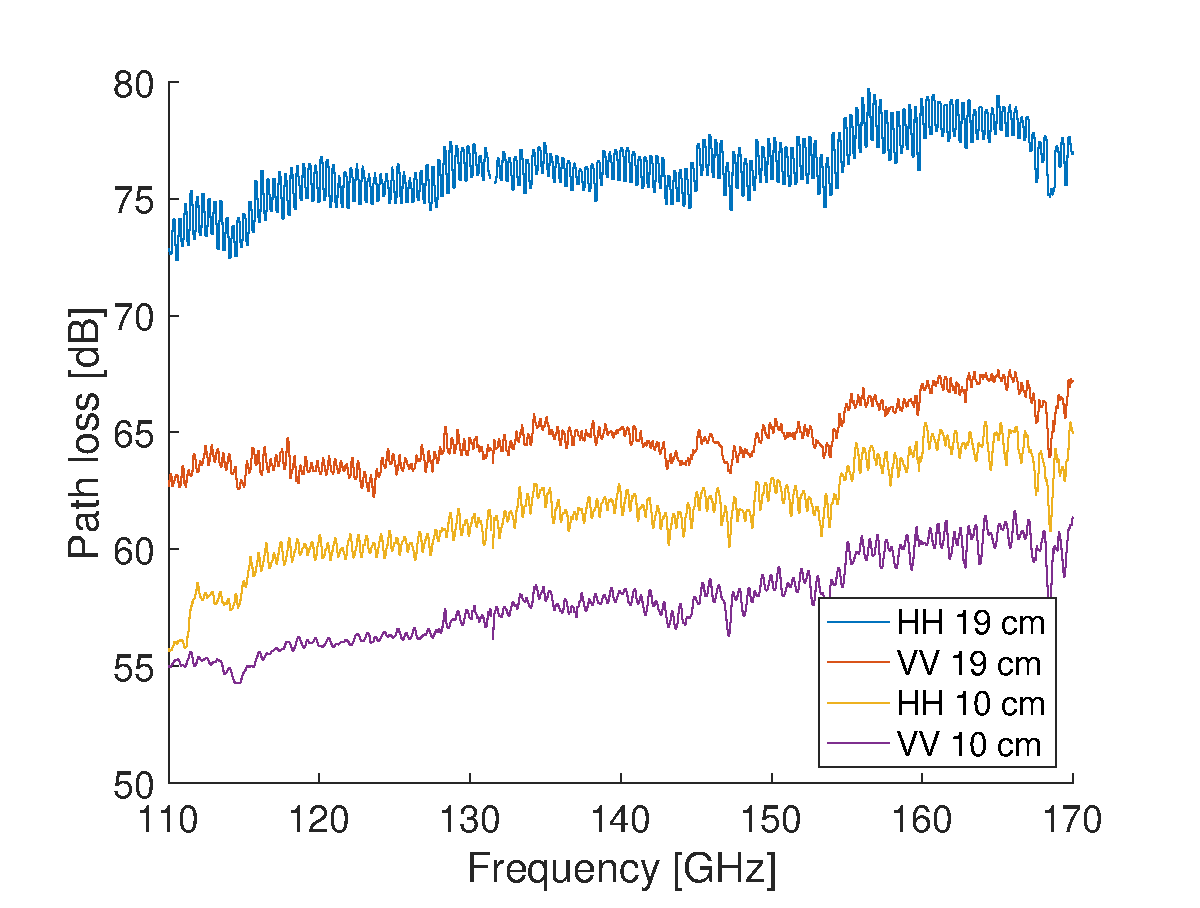
\includegraphics[width=0.45\textwidth]{figures/PL_vs_freq}
\caption{Measured path loss (PL) as a function of frequency for an antenna height of 1~mm above the skin phantom, antenna separations 10 and 19~cm, and vertical (VV) and horizontal (HH) co-polarizations.}
\label{fig:PL_vs_freq}
\end{center}
\end{figure}
The measured PL is higher than FSPL, due to absorption of radiated electromagnetic power by the skin phantom.
The highest PL is measured for the lowest height of 1~mm above the skin phantom.
Moreover, measured PL for horizontal co-polarized antennas (HH) is higher than for vertically polarized antennas (VV).
This is in line with the HPBW of the used antennas; the H-plane HPBW is larger than the E-plane HPBW and therefore, more radiated power is absorbed by the phantom in the horizontal co-polarized antenna setup.

Fitting the measurement data to the ABG model from (\ref{eq:ABG}) results in the fitted parameters listed in Table~\ref{table:ABG}. 
Both the PL exponent $\beta$ and frequency-dependence $\gamma$ are smaller than the free space value of 2. 
The p-values of all fitted parameters are below the significance level of 10$^{-3}$. 
Two aspects explain the low values for $\beta$ and $\gamma$, compared to the higher PL exponents ranging from 2 to 5 that are reported at millimeter-wave frequencies \cite{Petrillo2014, Aminzadeh2021_tap}. 
First, measurements are performed for very small antenna separations at which near-field effects need to be considered, whereas, the PL calculation in (\ref{eq:PL}) considers the far-field antenna gain.
Therefore, high PL values are obtained for smaller distances, which results in the smaller slope, i.e., a high reference PL $\alpha$ and low fitted values for $\beta$ and $\gamma$.
\begin{table}[tb]
  \caption{Fitted parameters of the ABG model for different polarizations (P) and antenna heights (H) above the skin phantom.}
  \label{table:ABG}
  \begin{center}
    \begin{tabular}{cc|cccc}
      P & H [mm] & $\alpha$ & $\beta$ & $\gamma$ & RMSE \\
      \hline
      VV & 1 & 44.6 dB & 0.54 & 0.48 & 2.7~dB \\
      VV & 3 & 38.0 dB & 0.81 & 0.62 & 3.3~dB \\
      VV & 6 & 41.2 dB & 0.65 & 0.54 & 2.6~dB \\
      HH & 1 & 26.6~dB & 3.13 & 0.30 & 3.0~dB \\
      HH & 3 & 44.5~dB & 0.68 & 0.36 & 2.3~dB \\
      HH & 6 & 45.5~dB & 0.60 & 0.34 & 2.2~dB \\
    \end{tabular}
  \end{center}
\end{table}

\subsection{Wideband path loss}

Figure~\ref{fig:PDP} shows the PDP for some select measurement scenarios. 
It is clear that round-trip reflections, i.e., reflections on the TX and RX antennas, are present.
These reflections cause a pulse to spread in time.
\begin{figure}[b!]
\begin{center}
	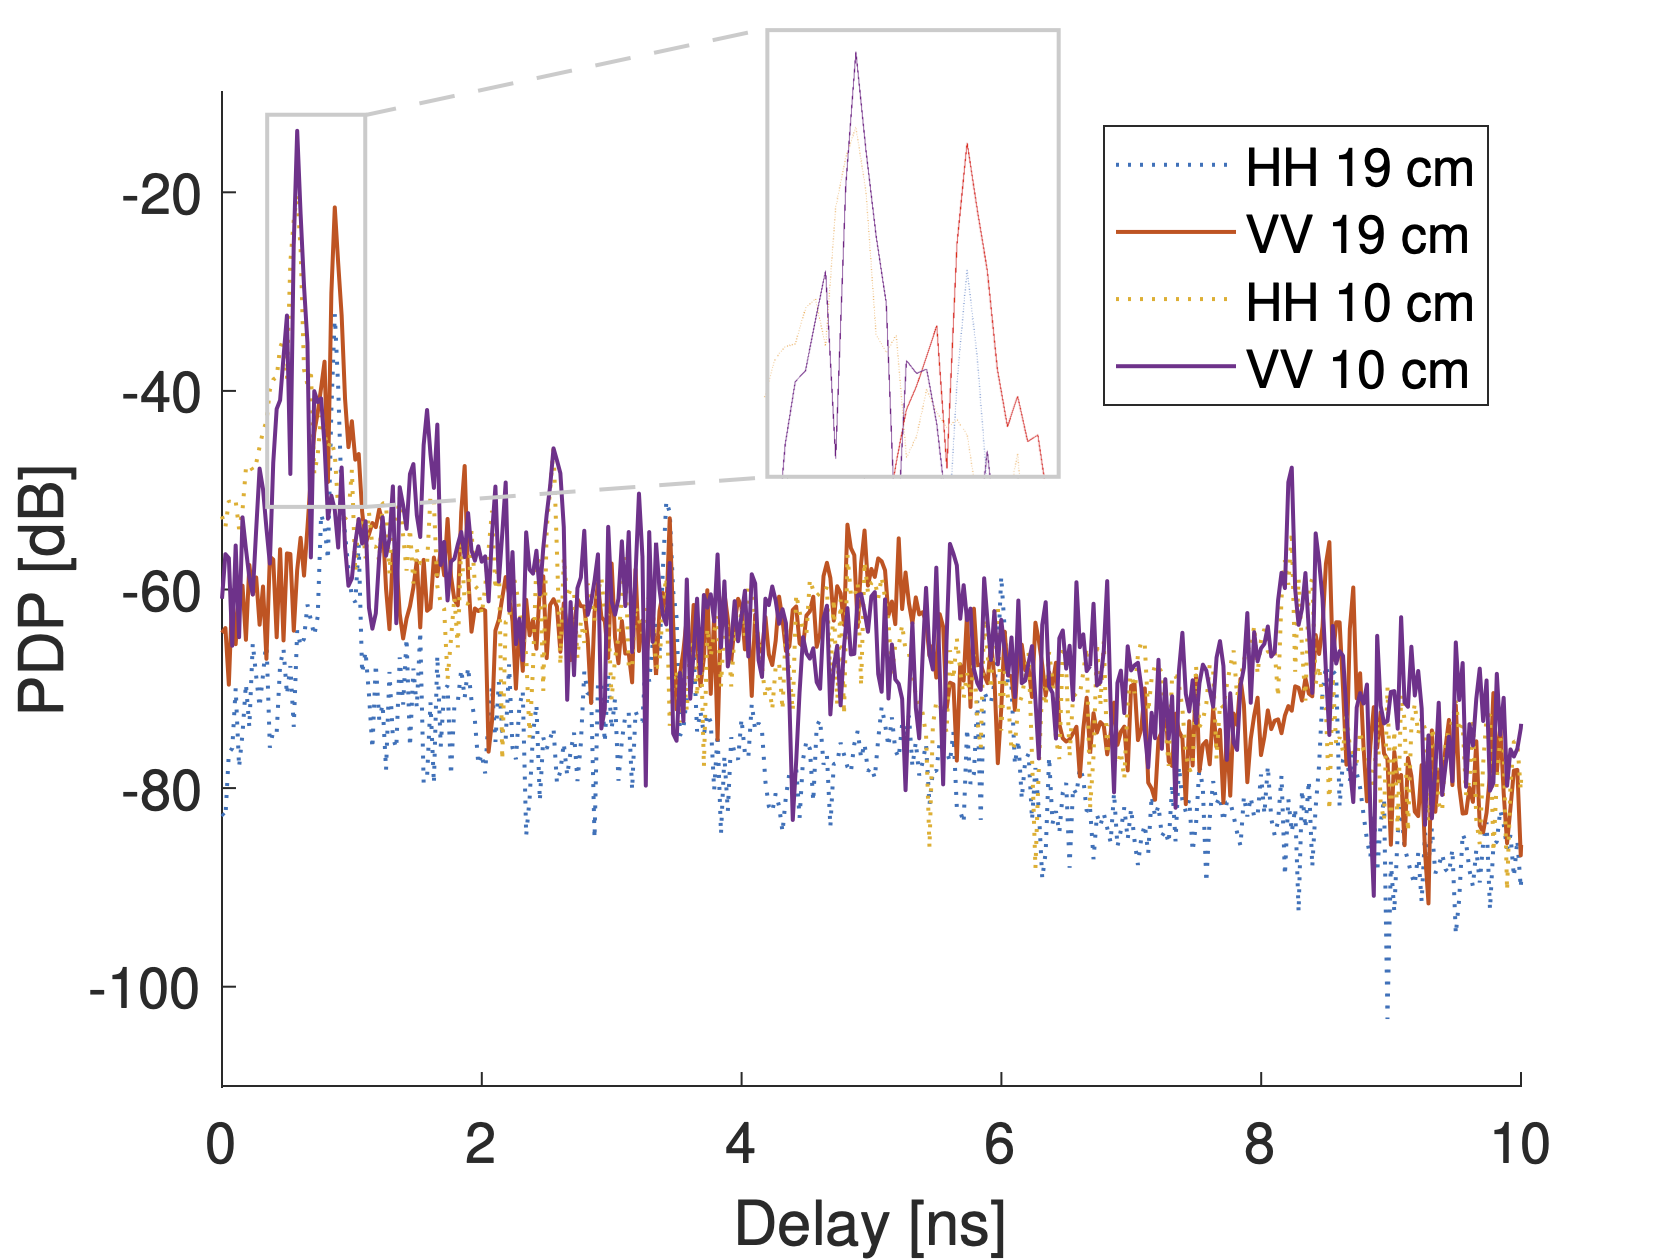
\includegraphics[width=0.45\textwidth]{figures/PDP}
\caption{Measured power delay profile (PDP) for different antenna separations and polarizations, with the antennas placed at 1~mm above the skin phantom.}
\label{fig:PDP}
\end{center}
\end{figure}
The reflections on the skin phantom cannot be resolved in the PDP, as the direct and reflected path lengths differ by less than 5~mm.

Wideband PL is obtained by selecting the power of the first peak and converting it into PL via (\ref{eq:WB-PL}). 
The measured PL as a function of distance is shown in Fig.~\ref{fig:PL_vs_dist}. 
\begin{figure}[tb]
\begin{center}
	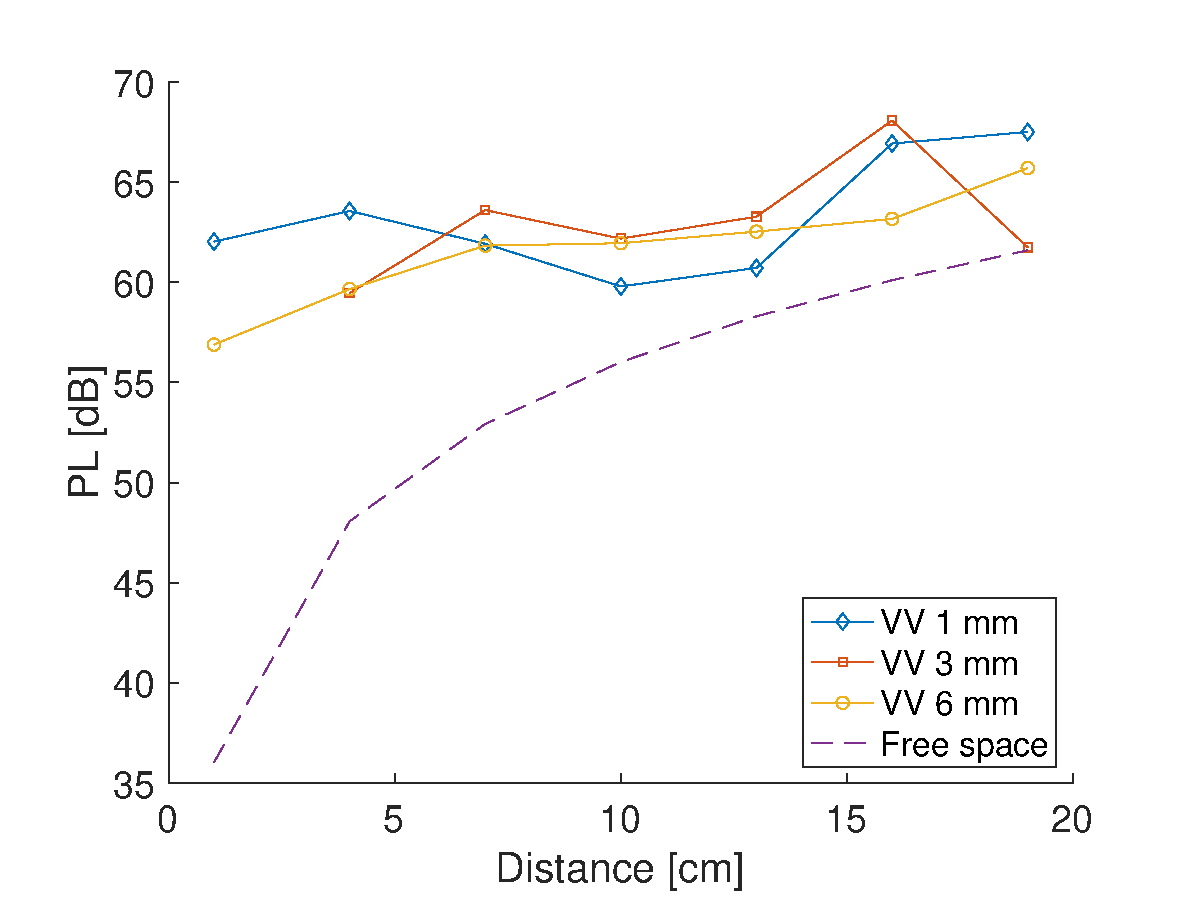
\includegraphics[width=0.45\textwidth]{figures/PL_vs_dist_VV}
	\\
	(a) VV
	\\
	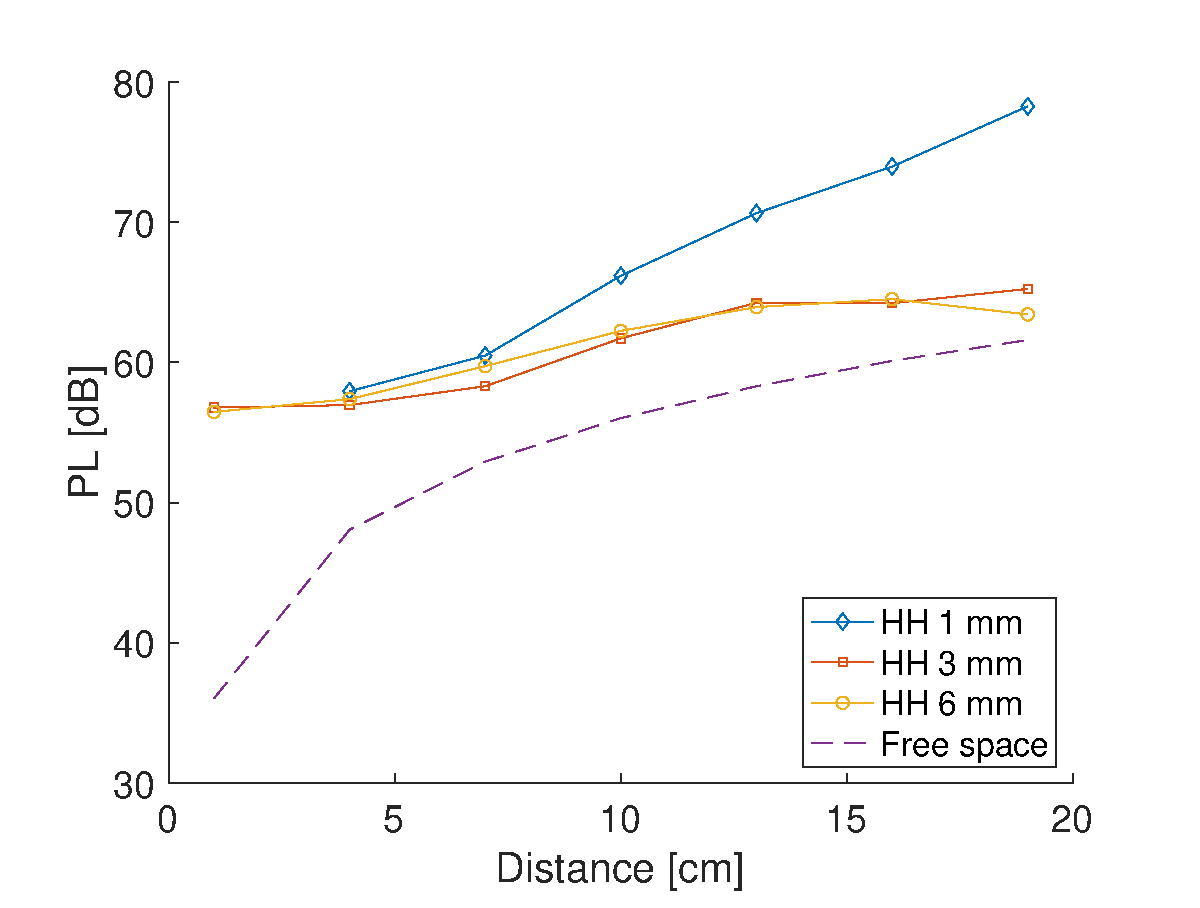
\includegraphics[width=0.45\textwidth]{figures/PL_vs_dist_HH}
	\\
	(b) HH
\caption{Measured wideband PL as a function of distance for different antenna heights.}
\label{fig:PL_vs_dist}
\end{center}
\end{figure}
From this figure, the small distance-dependence of PL is clear, which is in line with the low PL exponent $\beta$ from Table~\ref{table:ABG}.
Table~\ref{table:FI} lists the fitted parameters of the FI PL model from (\ref{eq:FI}).
In this case, the p-value of the PL exponent for VV polarization and antenna heights of 1 and 3~mm is above the 0.05 threshold.
\begin{table}[tb]
  \caption{Fitted parameters of the FI model for different polarizations (P) and antenna heights (H) above the skin phantom.}
  \label{table:FI}
  \begin{center}
    \begin{tabular}{cc|cccc}
      P & H [mm] & PL$_0$ & n& RMSE \\
      \hline
      VV & 1 & 61.1 dB & 0.25 & 3.0~dB \\
      VV & 3 & 56.6 dB & 0.65 & 2.6~dB \\
      VV & 6 & 56.5 dB & 0.60 & 0.9~dB \\
      HH & 1 & 37.3 dB & 3.04 & 2.2~dB \\
      HH & 3 & 54.8 dB & 0.72 & 2.0~dB \\
      HH & 6 & 55.3~dB & 0.67 & 1.4~dB \\
    \end{tabular}
  \end{center}
\end{table}

The difference between measured PL and FSPL is higher for small distances, due to a bad performance of the antennas, i.e., they are too close for efficient radiation. 
Even though the antennas are still in the near field, the measured PL is closer to FSPL for larger distances. 
Due to the high PL for small distances, both the ABG and FI models result in a PL exponent well below 2, with a reference PL above FSPL. 
PL is lower when the antennas are placed at a higher height above the skin phantom. 

\section{Conclusions\label{sect:conclusion}}

In this letter, an on-body measurement campaign is presented at D-band frequencies, ranging from 110 to 170~GHz. 
The influence of distance, frequency, antenna height above the skin phantom, and polarization are investigated.
With an increased frequency, and using waveguide-based antennas, the far-field distance of the antennas increases, and the antennas do not radiate efficiently at small antenna separations, resulting in a high measured path loss. 
Furthermore, when the antennas are placed above a skin, the boundary conditions are unfavorable for H-polarization due to current cancelation, and the mirror-effect can case interference in the V-polarization.
Both effects result in a path loss model with a high reference path loss and low path loss exponent.
The PL is higher when the height above the phantom is lower, and for a horizontally co-polarized antenna setup. 
The latter is caused by the larger half-power beamwidth of the antennas in the H-plane.

Future work includes the characterization of the skin phantom at D-band frequencies and the validation of the PL models on a real human body, also taking into account antenna mismatch, e.g., caused by wrist rotation.
Furthermore, a joint antenna and channel model is required, i.e., the antenna and channel characteristics need to be evaluated jointly as the antenna cannot be de-embedded from the measurements via the characteristics that are typically presented in the datasheet.

\section{Acknowledgment}

This work was executed within the imec AAA D-band channel modeling research project (D-BARC) and EOS project multi-service wireless network (MUSE-WINET). 

\vspace{3pt}

\suppressfloats
\bibliographystyle{IEEEtran}
\bibliography{RSL_140GHz_body}
\suppressfloats

\vspace{7pt}

%
% Note that the authors' affiliations and contact information should be
% here, after the references.
%
\noindent\small
B. De Beelde, A. Thielens, and W. Joseph are with Ghent University/IMEC, Department of Information Technology, Ghent, Belgium. 
R. Aminzadeh is with Unitron Group. 
Corresponding author: B. De Beelde. 
E-mail:Brecht.DeBeelde@gmail.com
\end{document}
